\documentclass[aspectratio=169,12pt,t]{beamer}
\usepackage{graphicx}
\setbeameroption{hide notes}
\setbeamertemplate{note page}[plain]
\usepackage{listings}
\usepackage{eepic}

% header.tex: boring LaTeX/Beamer details + macros

% get rid of junk
\usetheme{default}
\beamertemplatenavigationsymbolsempty
\hypersetup{pdfpagemode=UseNone} % don't show bookmarks on initial view


% font
\usepackage{fontspec}
\setsansfont
  [ ExternalLocation = ../fonts/ ,
    UprightFont = *-regular ,
    BoldFont = *-bold ,
    ItalicFont = *-italic ,
    BoldItalicFont = *-bolditalic ]{texgyreheros}
\setbeamerfont{note page}{family*=pplx,size=\footnotesize} % Palatino for notes
% "TeX Gyre Heros can be used as a replacement for Helvetica"
% I've placed them in fonts/; alternatively you can install them
% permanently on your system as follows:
%     Download http://www.gust.org.pl/projects/e-foundry/tex-gyre/heros/qhv2.004otf.zip
%     In Unix, unzip it into ~/.fonts
%     In Mac, unzip it, double-click the .otf files, and install using "FontBook"

% named colors
\definecolor{offwhite}{RGB}{255,250,240}
\definecolor{gray}{RGB}{155,155,155}
\definecolor{purple}{RGB}{177,13,201}
\definecolor{green}{RGB}{46,204,64}

\definecolor{background}{RGB}{255,255,255}
\definecolor{foreground}{RGB}{24,24,24}
\definecolor{title}{RGB}{27,94,134}
\definecolor{subtitle}{RGB}{22,175,124}
\definecolor{hilit}{RGB}{122,0,128}
\definecolor{vhilit}{RGB}{255,0,128}
\definecolor{codehilit}{RGB}{255,0,128}
\definecolor{lolit}{RGB}{95,95,95}
\definecolor{myyellow}{rgb}{1,1,0.7}
\definecolor{nhilit}{RGB}{128,0,128}  % hilit color in notes
\definecolor{nvhilit}{RGB}{255,0,128} % vhilit for notes

\newcommand{\hilit}{\color{hilit}}
\newcommand{\vhilit}{\color{vhilit}}
\newcommand{\nhilit}{\color{nhilit}}
\newcommand{\nvhilit}{\color{nvhilit}}
\newcommand{\lolit}{\color{lolit}}

% use those colors
\setbeamercolor{titlelike}{fg=title}
\setbeamercolor{subtitle}{fg=subtitle}
\setbeamercolor{institute}{fg=lolit}
\setbeamercolor{normal text}{fg=foreground,bg=background}
\setbeamercolor{item}{fg=foreground} % color of bullets
\setbeamercolor{subitem}{fg=lolit}
\setbeamercolor{itemize/enumerate subbody}{fg=lolit}
\setbeamertemplate{itemize subitem}{{\textendash}}
\setbeamerfont{itemize/enumerate subbody}{size=\footnotesize}
\setbeamerfont{itemize/enumerate subitem}{size=\footnotesize}

% page number
\setbeamertemplate{footline}{%
    \raisebox{5pt}{\makebox[\paperwidth]{\hfill\makebox[20pt]{\lolit
          \scriptsize\insertframenumber}}}\hspace*{5pt}}

% add a bit of space at the top of the notes page
\addtobeamertemplate{note page}{\setlength{\parskip}{12pt}}

% default link color
\hypersetup{colorlinks, urlcolor={hilit}}

\lstset{language=bash,
        basicstyle=\ttfamily\scriptsize,
        frame=single,
        commentstyle=,
        backgroundcolor=\color{offwhite},
        showspaces=false,
        showstringspaces=false
        }


% a few macros
\newcommand{\bi}{\begin{itemize}}
\newcommand{\bbi}{\vspace{24pt} \begin{itemize} \itemsep8pt}
\newcommand{\ei}{\end{itemize}}
\newcommand{\be}{\begin{enumerate}}
\newcommand{\bbe}{\vspace{24pt} \begin{enumerate} \itemsep8pt}
\newcommand{\ee}{\end{enumerate}}
\newcommand{\ig}{\includegraphics}
\newcommand{\subt}[1]{{\footnotesize \color{subtitle} {#1}}}
\newcommand{\ttsm}{\tt \small}
\newcommand{\ttfn}{\tt \footnotesize}
\newcommand{\figh}[2]{\centerline{\includegraphics[height=#2\textheight]{#1}}}
\newcommand{\figw}[2]{\centerline{\includegraphics[width=#2\textwidth]{#1}}}


%%%%%%%%%%%%%%%%%%%%%%%%%%%%%%%%%%%%%%%%%%%%%%%%%%%%%%%%%%%%%%%%%%%%%%
% end of header
%%%%%%%%%%%%%%%%%%%%%%%%%%%%%%%%%%%%%%%%%%%%%%%%%%%%%%%%%%%%%%%%%%%%%%

% title info
\title{The EM algorithm}
\subtitle{QTL mapping with a cure model}
\author{\href{https://kbroman.org}{Karl Broman}}
\institute{Biostatistics \& Medical Informatics, UW{\textendash}Madison}
\date{\href{https://kbroman.org}{\tt \scriptsize \color{foreground} kbroman.org}
\\[-4pt]
\href{https://github.com/kbroman}{\tt \scriptsize \color{foreground} github.com/kbroman}
\\[-4pt]
\href{https://twitter.com/kwbroman}{\tt \scriptsize \color{foreground} @kwbroman}
\\[-4pt]
{\scriptsize Course web: \href{https://kbroman.org/AdvData}{\tt kbroman.org/AdvData}}
}


\begin{document}

% title slide
{
\setbeamertemplate{footline}{} % no page number here
\frame{
  \titlepage

  \note{}

} }



\begin{frame}[c]{Intercross}
\figw{Figs/intercross.pdf}{1.0}
\end{frame}





\begin{frame}[c]{QTL mapping}

\vspace{5mm}
\figw{Figs/lodcurve_insulin_with_effects.pdf}{0.96}
\end{frame}




\begin{frame}[c]{Phenotype data}
\figw{Figs/pheno.pdf}{1.0}

\vspace{5mm}

{\lolit \footnotesize
Sugiyama et al.\ (2002) Physiol Genomics 10:5--12
}
\end{frame}


\begin{frame}[c]{Genotype data}
\figw{Figs/genodata.pdf}{1.0}
\end{frame}


\begin{frame}[c]{Genetic map}
\figw{Figs/geneticmap.pdf}{1.0}
\end{frame}



\begin{frame}[c]{ANOVA at marker loci}

\begin{columns}

\column{0.5\textwidth}
\bi
\item Also known as {\hilit marker regression}.
\item Split mice into groups according to genotype at a marker.
\item Do a t-test / ANOVA.
\item Repeat for each marker.
\ei

\column{0.5\textwidth}

\figw{Figs/anova.pdf}{1.0}

\end{columns}
\end{frame}



\begin{frame}{ANOVA at marker loci}

\begin{columns}
\column{0.5\textwidth}

{\hilit Advantages}

\bi
\item Simple.
\item Easily incorporates covariates.
\item Easily extended to more complex models.
\item Doesn't require a genetic map.
\ei


\column{0.5\textwidth}

{\hilit Disadvantages}

\bi
\item Must exclude individuals with missing genotype data.
\item Imperfect information about QTL location.
\item Suffers in low density scans.
\item {\vhilit Only considers one QTL at a time.}
\ei

\end{columns}

\end{frame}




\begin{frame}{Interval mapping}

{\hilit Lander \& Botstein (1989)}

\bbi
  \item Assume a {\hilit single} QTL model.
  \item Each position in the genome, one at a time, is posited as the
  putative QTL.
  \item Let $\mathsf{q = }$ 0/1/2 if the (unobserved) QTL genotype is
  AA/AB/BB. \\[12pt]
        Assume $\mathsf{y | q \sim N(\mu_q, \sigma)}$
  \item Given genotypes at linked markers, $\mathsf{y \sim}$ mixture of normal
  dist'ns with mixing proportions $\mathsf{\text{Pr}(q \ | \ \text{marker data})}$
\ei

\end{frame}

\begin{frame}[c]{Backcross}
\figw{Figs/backcross.pdf}{1.0}
\end{frame}


\begin{frame}{Genotype probabilities}


\only<1>{\figw{Figs/genoprob1.pdf}{1.0}}
\only<2>{\figw{Figs/genoprob2.pdf}{1.0}}
\only<3>{\figw{Figs/genoprob3.pdf}{1.0}}
\only<4>{\figw{Figs/genoprob4.pdf}{1.0}}
\only<5>{\figw{Figs/genoprob5.pdf}{1.0}}
\only<6>{\figw{Figs/genoprob6.pdf}{1.0}}

\bigskip

{\small
Calculate {\hilit $\mathsf{\text{Pr}(q \ | \ \text{marker data})}$}, assuming

\sbi
\item No crossover interference
\item No genotyping errors
\ei

\bigskip

Or use the {\hilit hidden Markov model (HMM)} technology

\sbi
\item To allow for genotyping errors
\item To incorporate dominant markers
\item {\hilit (Still assume no crossover interference.)}
\ei
}

\end{frame}





\begin{frame}{The normal mixtures}

\vspace{-5mm}

\begin{columns}
\column{0.5\textwidth}

\setlength{\unitlength}{0.18\textwidth}
\begin{center}
\begin{picture}(4.5,1)
\small
% lines
\Thicklines
\put(0.25,0.5){\line(1,0){4}}
\put(0.25,0.35){\line(0,1){0.3}}
\put(1.65,0.35){\line(0,1){0.3}}
\put(4.25,0.35){\line(0,1){0.3}}

% text
\put(0.25,0.1){\makebox(0,0){$\mathsf{M_1}$}}
\put(4.25,0.1){\makebox(0,0){$\mathsf{M_2}$}}
\put(1.65,0.1){\makebox(0,0){$\mathsf{Q}$}}
\put(0.95,0.8){\makebox(0,0){7 cM}}
\put(2.95,0.8){\makebox(0,0){13 cM}}
\end{picture} \end{center}
\vspace{5mm}

\sbi
\itemsep18pt
\item Two markers separated by 20 cM, with the QTL closer to the left marker.
\item The figure at right shows the distributions of the phenotype
conditional on the genotypes at the two markers.
\item The dashed curves correspond to the components of the mixtures.
\ei


\column{0.5\textwidth}

\vspace*{-5mm}

\figw{Figs/mixtures.pdf}{1.0}

\end{columns}
\end{frame}





\begin{frame}[c]{Interval mapping}


  \bbi
  \itemsep18pt

\item[] Let $\mathsf{p_{ij} = \text{Pr}(q_i = j | \text{marker data})}$

\item[] $\mathsf{y_i | q_i \sim N(\mu_{q_i},\sigma^2)}$

\item[] $\mathsf{\text{Pr}(y_i | \text{marker data},\mu_0,\mu_1,\sigma) =
\sum_j p_{ij} \, f(y_i; \mu_j,\sigma)}$

\qquad where $\mathsf{f(y; \mu,\sigma)= \exp[-(y-\mu)^2/(2\sigma^2)] / \sqrt{2 \pi
\sigma^2}}$


\item[] {\hilit Log likelihood}: \hspace{5mm}
$\mathsf{l(\mu_0,\mu_1,\sigma) = \sum_i \log \text{Pr}(y_i | \text{marker
data},\mu_0,\mu_1,\sigma)}$

\item[] Maximum likelihood estimates ({\hilit MLEs})
of $\mathsf{\mu_0}$, $\mathsf{\mu_1}$, $\mathsf{\sigma}$:

\qquad values for which $\mathsf{l(\mu_0,\mu_1,\sigma)}$ is maximized.
\ei

\end{frame}




\begin{frame}{EM algorithm}


\vspace*{-8mm}
\bbi

\item[] {\hilit E step}:

\qquad Let \hspace{5mm} $w_{ij}^{(k)} = \text{Pr}(q_i = j |
y_i,\text{marker data},\hat{\mu}_0^{(k-1)},
\hat{\mu}_1^{(k-1)},\hat{\sigma}^{(k-1)})$ \\[12pt]

\hspace{29mm} $ = \frac{p_{ij} \, f(y_i; \hat{\mu}_j^{(k-1)},\hat{\sigma}^{(k-1)})}{ \sum_j p_{ij} \, f(y_i; \hat{\mu}_j^{(k-1)},\hat{\sigma}^{(k-1)})}$


\item[] {\hilit M step}:

\qquad Let \hspace{5mm} $\hat{\mu}_j^{(k)} = \sum_i y_i w_{ij}^{(k)} /
\sum_i w_{ij}^{(k)}$ \\[12pt]

\hspace{20mm} $\hat{\sigma}^{(k)} = \sqrt{ \sum_i \sum_j w_{ij}^{(k)} (y_i-\hat{\mu}_j^{(k)})^2/n}$


\item[] {\hilit The algorithm}: \\[6pt]

\qquad Start with $w_{ij}^{(1)} = p_{ij}$; iterate the E \& M steps until convergence.

\ei

\end{frame}



\begin{frame}[c]{\href{http://www.biostat.wisc.edu/~kbroman/D3/em_alg/}{Interactive illustration}}

\centerline{\href{http://www.biostat.wisc.edu/~kbroman/D3/em_alg/}{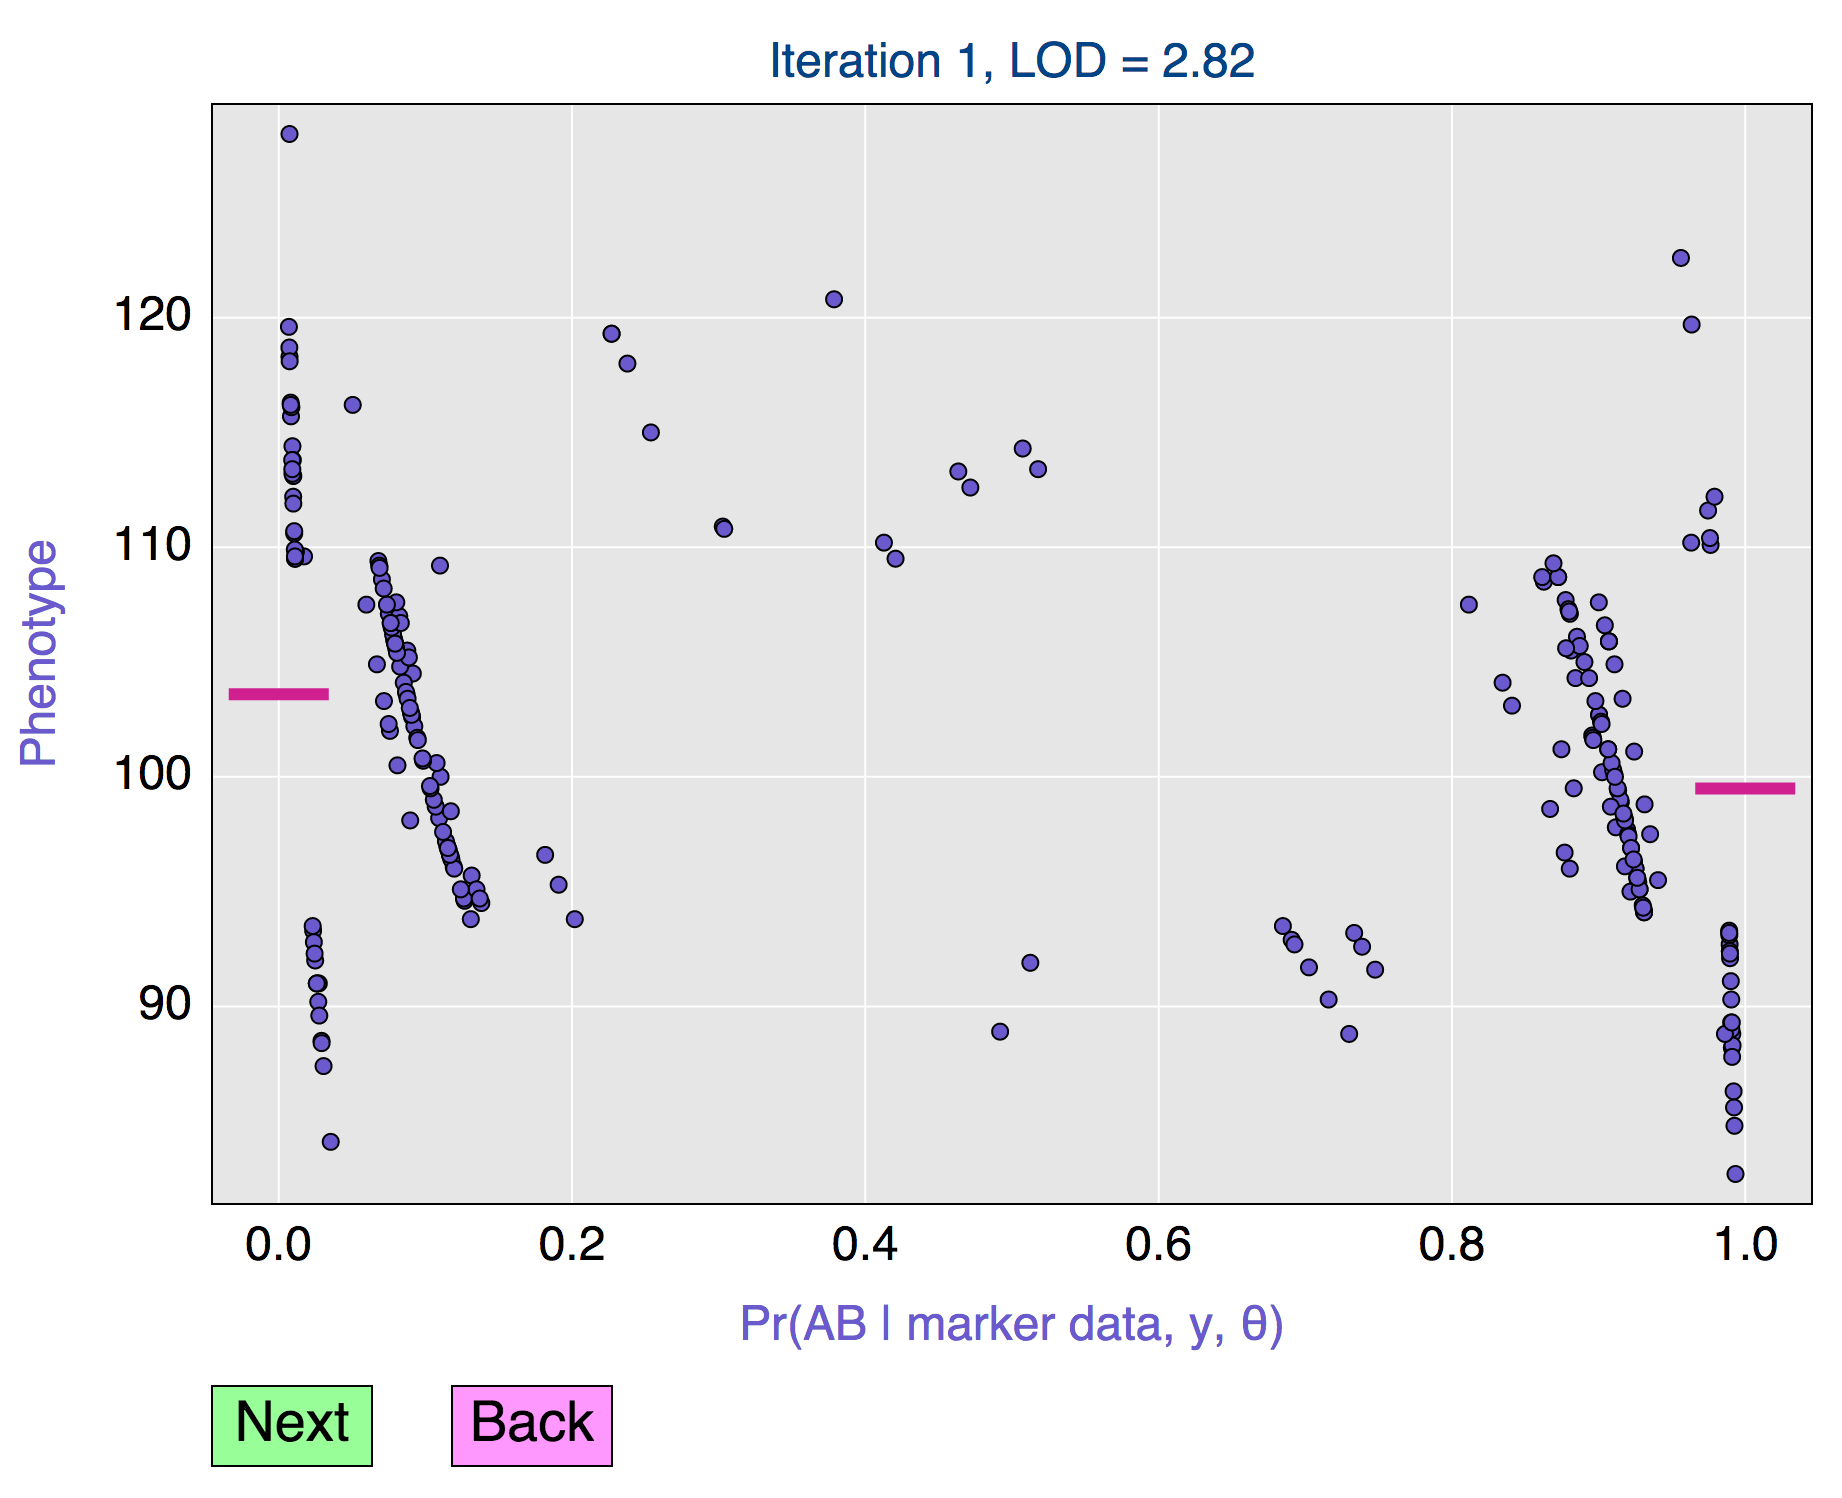
\includegraphics[width=0.7\textwidth]{Figs/em_alg_illustration.png}}}

\end{frame}



\begin{frame}[c]{LOD scores}

 The LOD score is a measure of the {\hilit strength of
evidence} for the presence of a QTL at a particular
location.

\bbi
\itemsep18pt

\item[] $\text{LOD}(\lambda) = \log_{10}$ likelihood ratio comparing the hypothesis of a \\

\hspace{25mm} QTL at position $\lambda$ versus that of no QTL \\[8pt]

\hspace{14mm} $= \log_{10} \left\{ \frac{\text{Pr}(y | \text{QTL at $\lambda$}, \hat{\mu}_{0\lambda},
\hat{\mu}_{1\lambda}, \hat{\sigma}_\lambda)}{\text{Pr}(y | \text{no QTL}, \hat{\mu},
\hat{\sigma})} \right\}$

 \item[] $\hat{\mu}_{0\lambda}, \hat{\mu}_{1\lambda}, \hat{\sigma}_\lambda$ are the MLEs,
assuming a single QTL at position $\lambda$.


 \item[] {\hilit No QTL model:}

\bi
  \item[] {\color{foreground} The phenotypes are independent and identically
distributed (iid) $\text{N}(\mu, \sigma^2)$}.
\ei

\ei

\end{frame}





\begin{frame}[c]{\href{http://www.biostat.wisc.edu/~kbroman/D3/lod_and_effect/}{Interactive plot}}

\centerline{\href{http://www.biostat.wisc.edu/~kbroman/D3/lod_and_effect/}{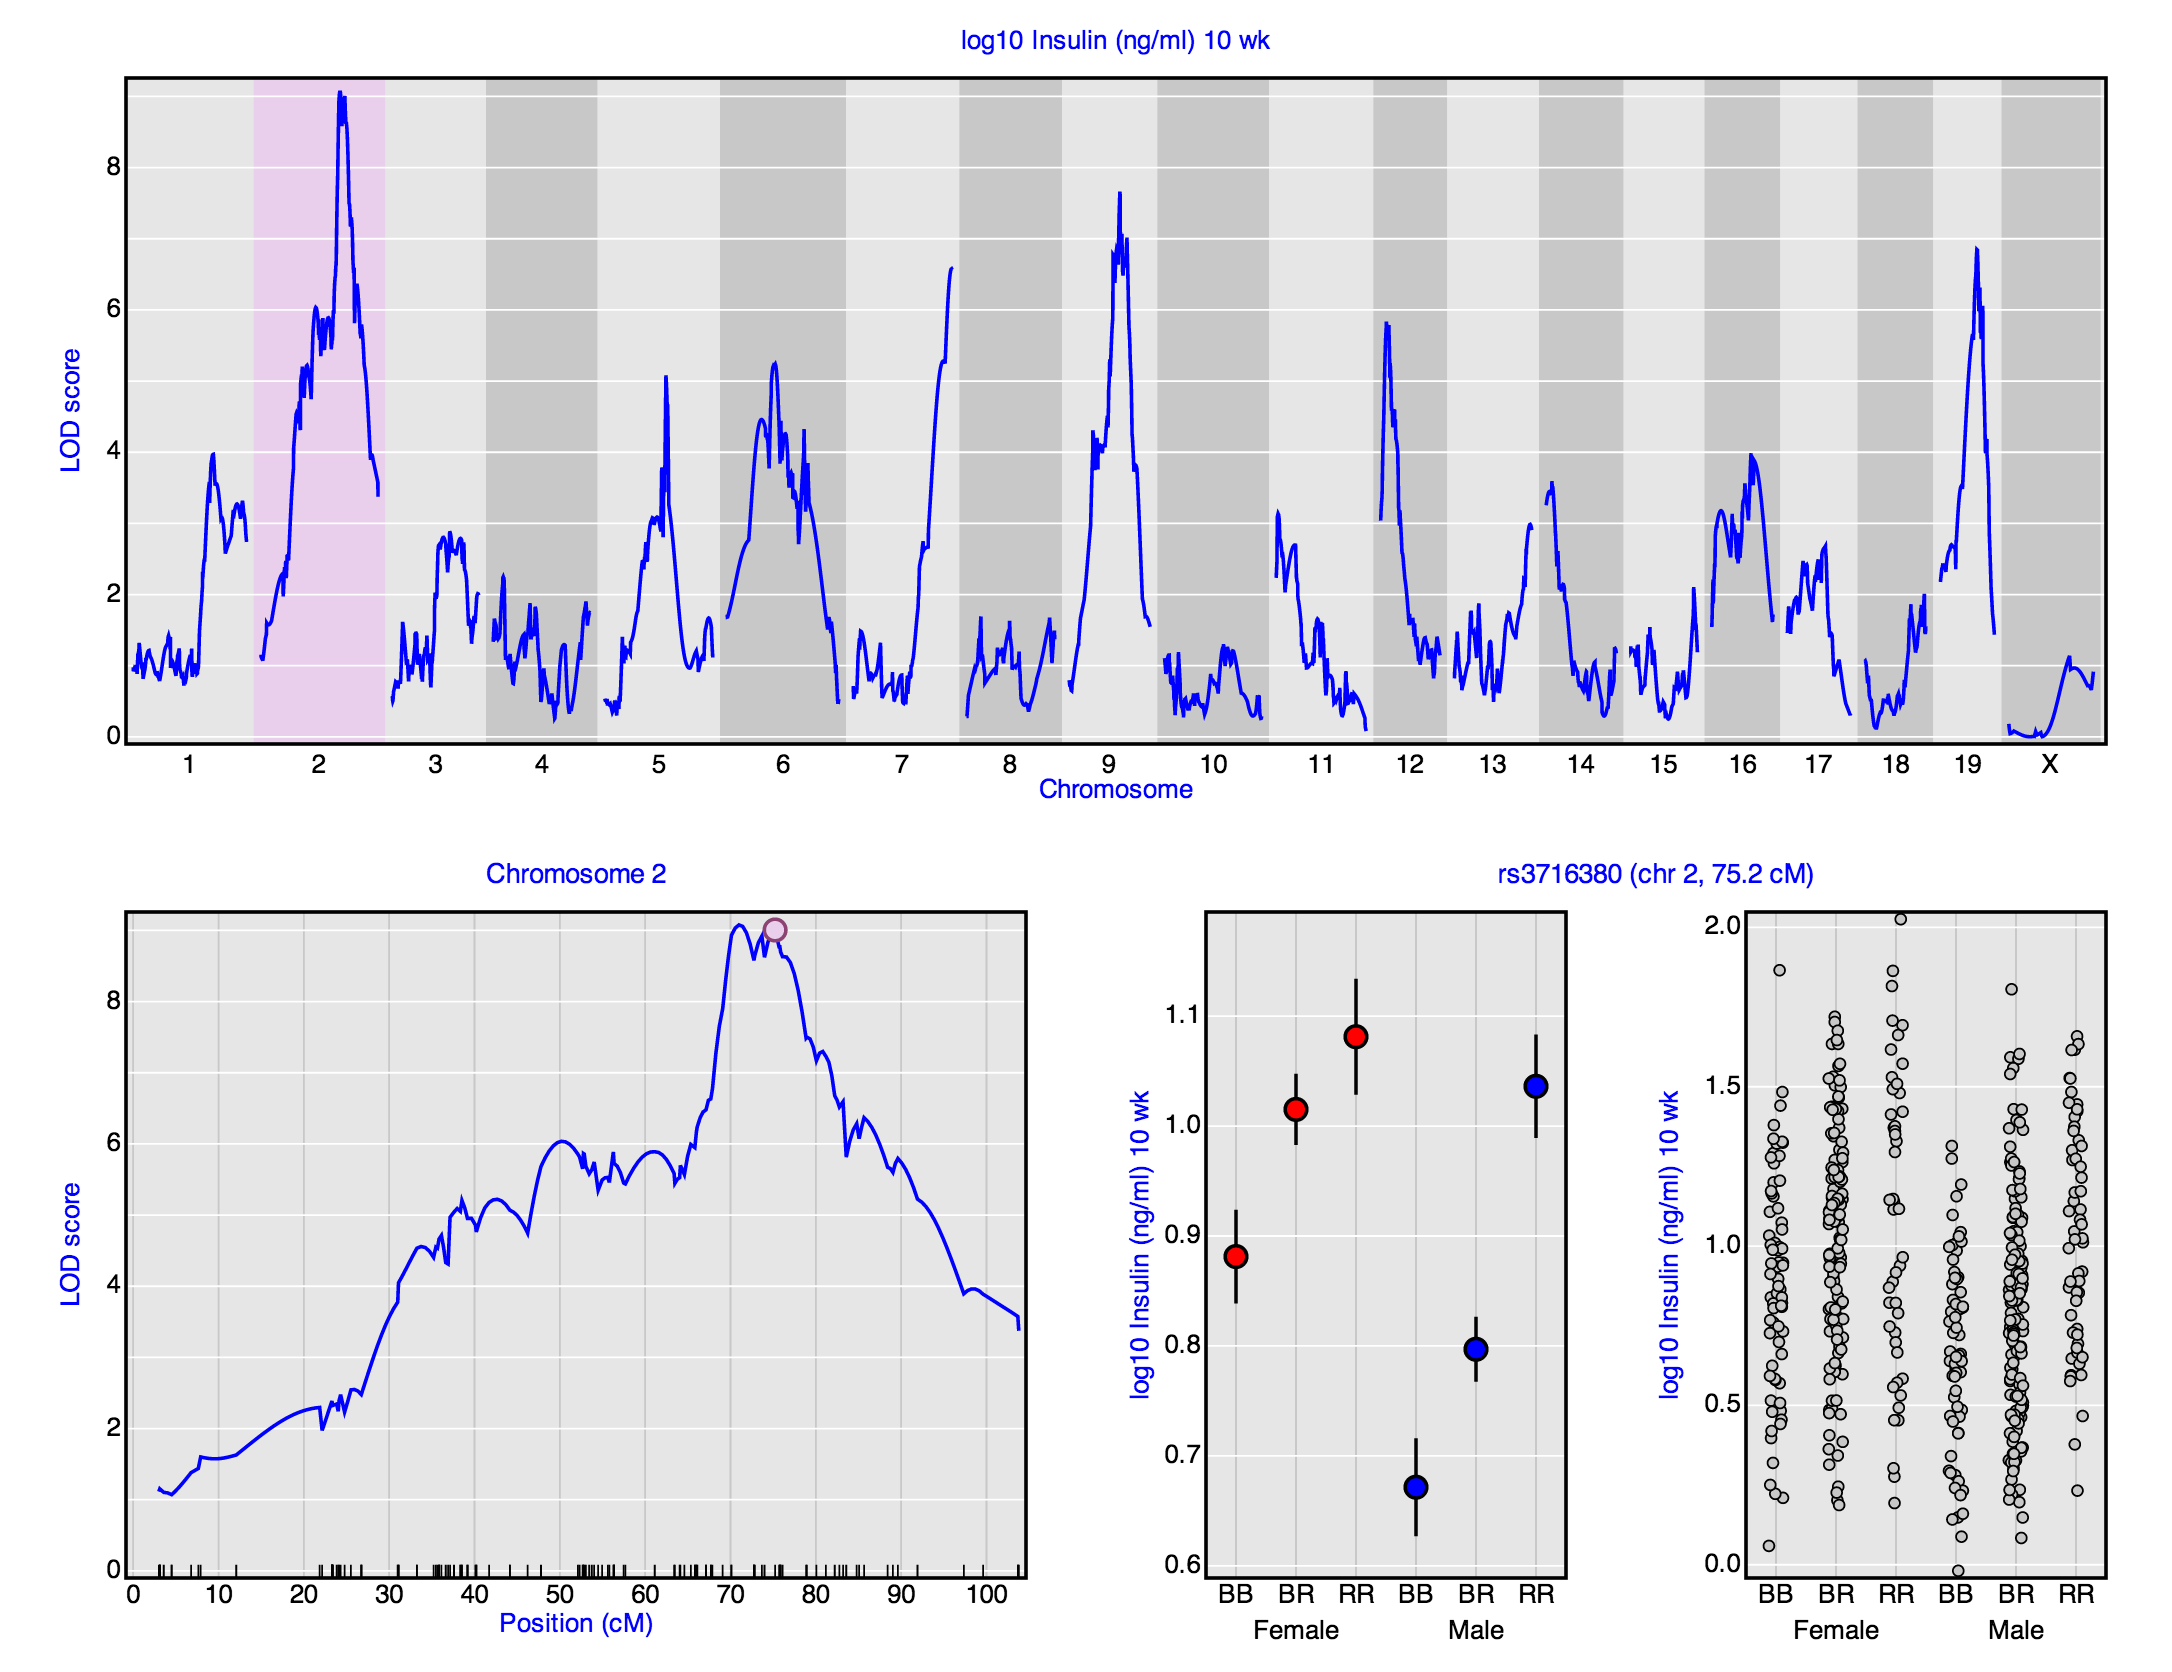
\includegraphics[width=0.75\textwidth]{Figs/interactive_lod_curve.png}}}

\end{frame}





\begin{frame}{Interval mapping}

\begin{columns}

\column{0.5\textwidth}

{\hilit Advantages}

\bi
\item Takes proper account of missing data.
\item Allows examination of positions between markers.
\item Gives improved estimates of QTL effects.
\item Provides pretty graphs.
\ei


\column{0.5\textwidth}

{\hilit Disadvantages}

\bi
\item Increased computation time.
\item Requires specialized software.
\item Difficult to generalize.
\item {\vhilit Only considers one QTL at a time.}
\ei


\end{columns}

\end{frame}



\begin{frame}{References}
\vspace{-7mm}

  \bbi

\item Lander ES, Botstein D (1989) Mapping Mendelian factors
  underlying quantitative traits using RFLP linkage maps. Genetics
  121:185-199 \\
  \href{https://www.ncbi.nlm.nih.gov/pmc/articles/PMC1203601}{\footnotesize
    PMCID: PMC1203601}

\item Broman KW (2001) Review of statistical methods for QTL mapping
  in experimental crosses. Lab Animal 30(7):44-52 \\
  \href{https://www.ncbi.nlm.nih.gov/pubmed/11469113}{\footnotesize
    PMID: 11469113}

\item Boyartchuk VL, et al. (2001) Multigenic control of Listeria monocytogenes
  susceptibility in mice. Nat Genet 27:259-260 \\
  \href{https://doi.org/10.1038/85812}{\footnotesize doi:10.1038/85812}

\item Broman KW (2003) Mapping quantitative trait loci in the case
  of a spike in the phenotype distribution. Genetics 163:1169-1175 \\
  \href{https://www.ncbi.nlm.nih.gov/pmc/articles/PMC1462498}{\footnotesize
    PMCID: PMC1462498}

\ei


\end{frame}


\end{document}
